\documentclass[a4paper, 10pt]{article}
\usepackage[english,brazil]{babel}
\usepackage[utf8]{inputenc}
\usepackage{fullpage}
\usepackage{float}

% \usepackage{multicol}
\usepackage{graphicx}
\usepackage{listings}
% \setlength{\columnsep}{30pt}
% I want the columnsep to be wider only on this page. Right now, nothing happens. The default 10pt is still being used.

\lstdefinestyle{cppStyle}{
  basicstyle=\footnotesize,
  breakatwhitespace=false,
  breaklines=true,
  captionpos=b,
  keepspaces=true,
  numbers=left,
  numbersep=5pt,
  showspaces=false,
  showstringspaces=false,
  showtabs=false,
  tabsize=2
}

\renewcommand*{\lstlistingname}{Código}

\newcounter{codeNum}
\setcounter{codeNum}{0}

\begin{document}

\noindent
\large
\textbf{Compiladores} \\
\textbf{1ª Série de Exercícios} \\
\normalsize CES-41  \\
Professor: Fábio Carneiro Mokarzel \\
Aluno: Carlos Matheus Barros da Silva \hfill Julho de 2019 \\ \\


%-------------------------------------------------------------------------------
Todos os códigos desta lista podem ser acessados no repositório do GitHub:

\textit{https://github.com/CarlosMatheus/CES-41-Exercise-Lists}

\section*{Exercício 1}

O Exercicio foi resolvido com sucesso. Seu funcionamento pode ser observado pela saída representada pelo Código \ref{code:saida} que é referente a entrada representada no Código \ref{code:entrada}.

\begin{figure}[H]
  \begin{center}
  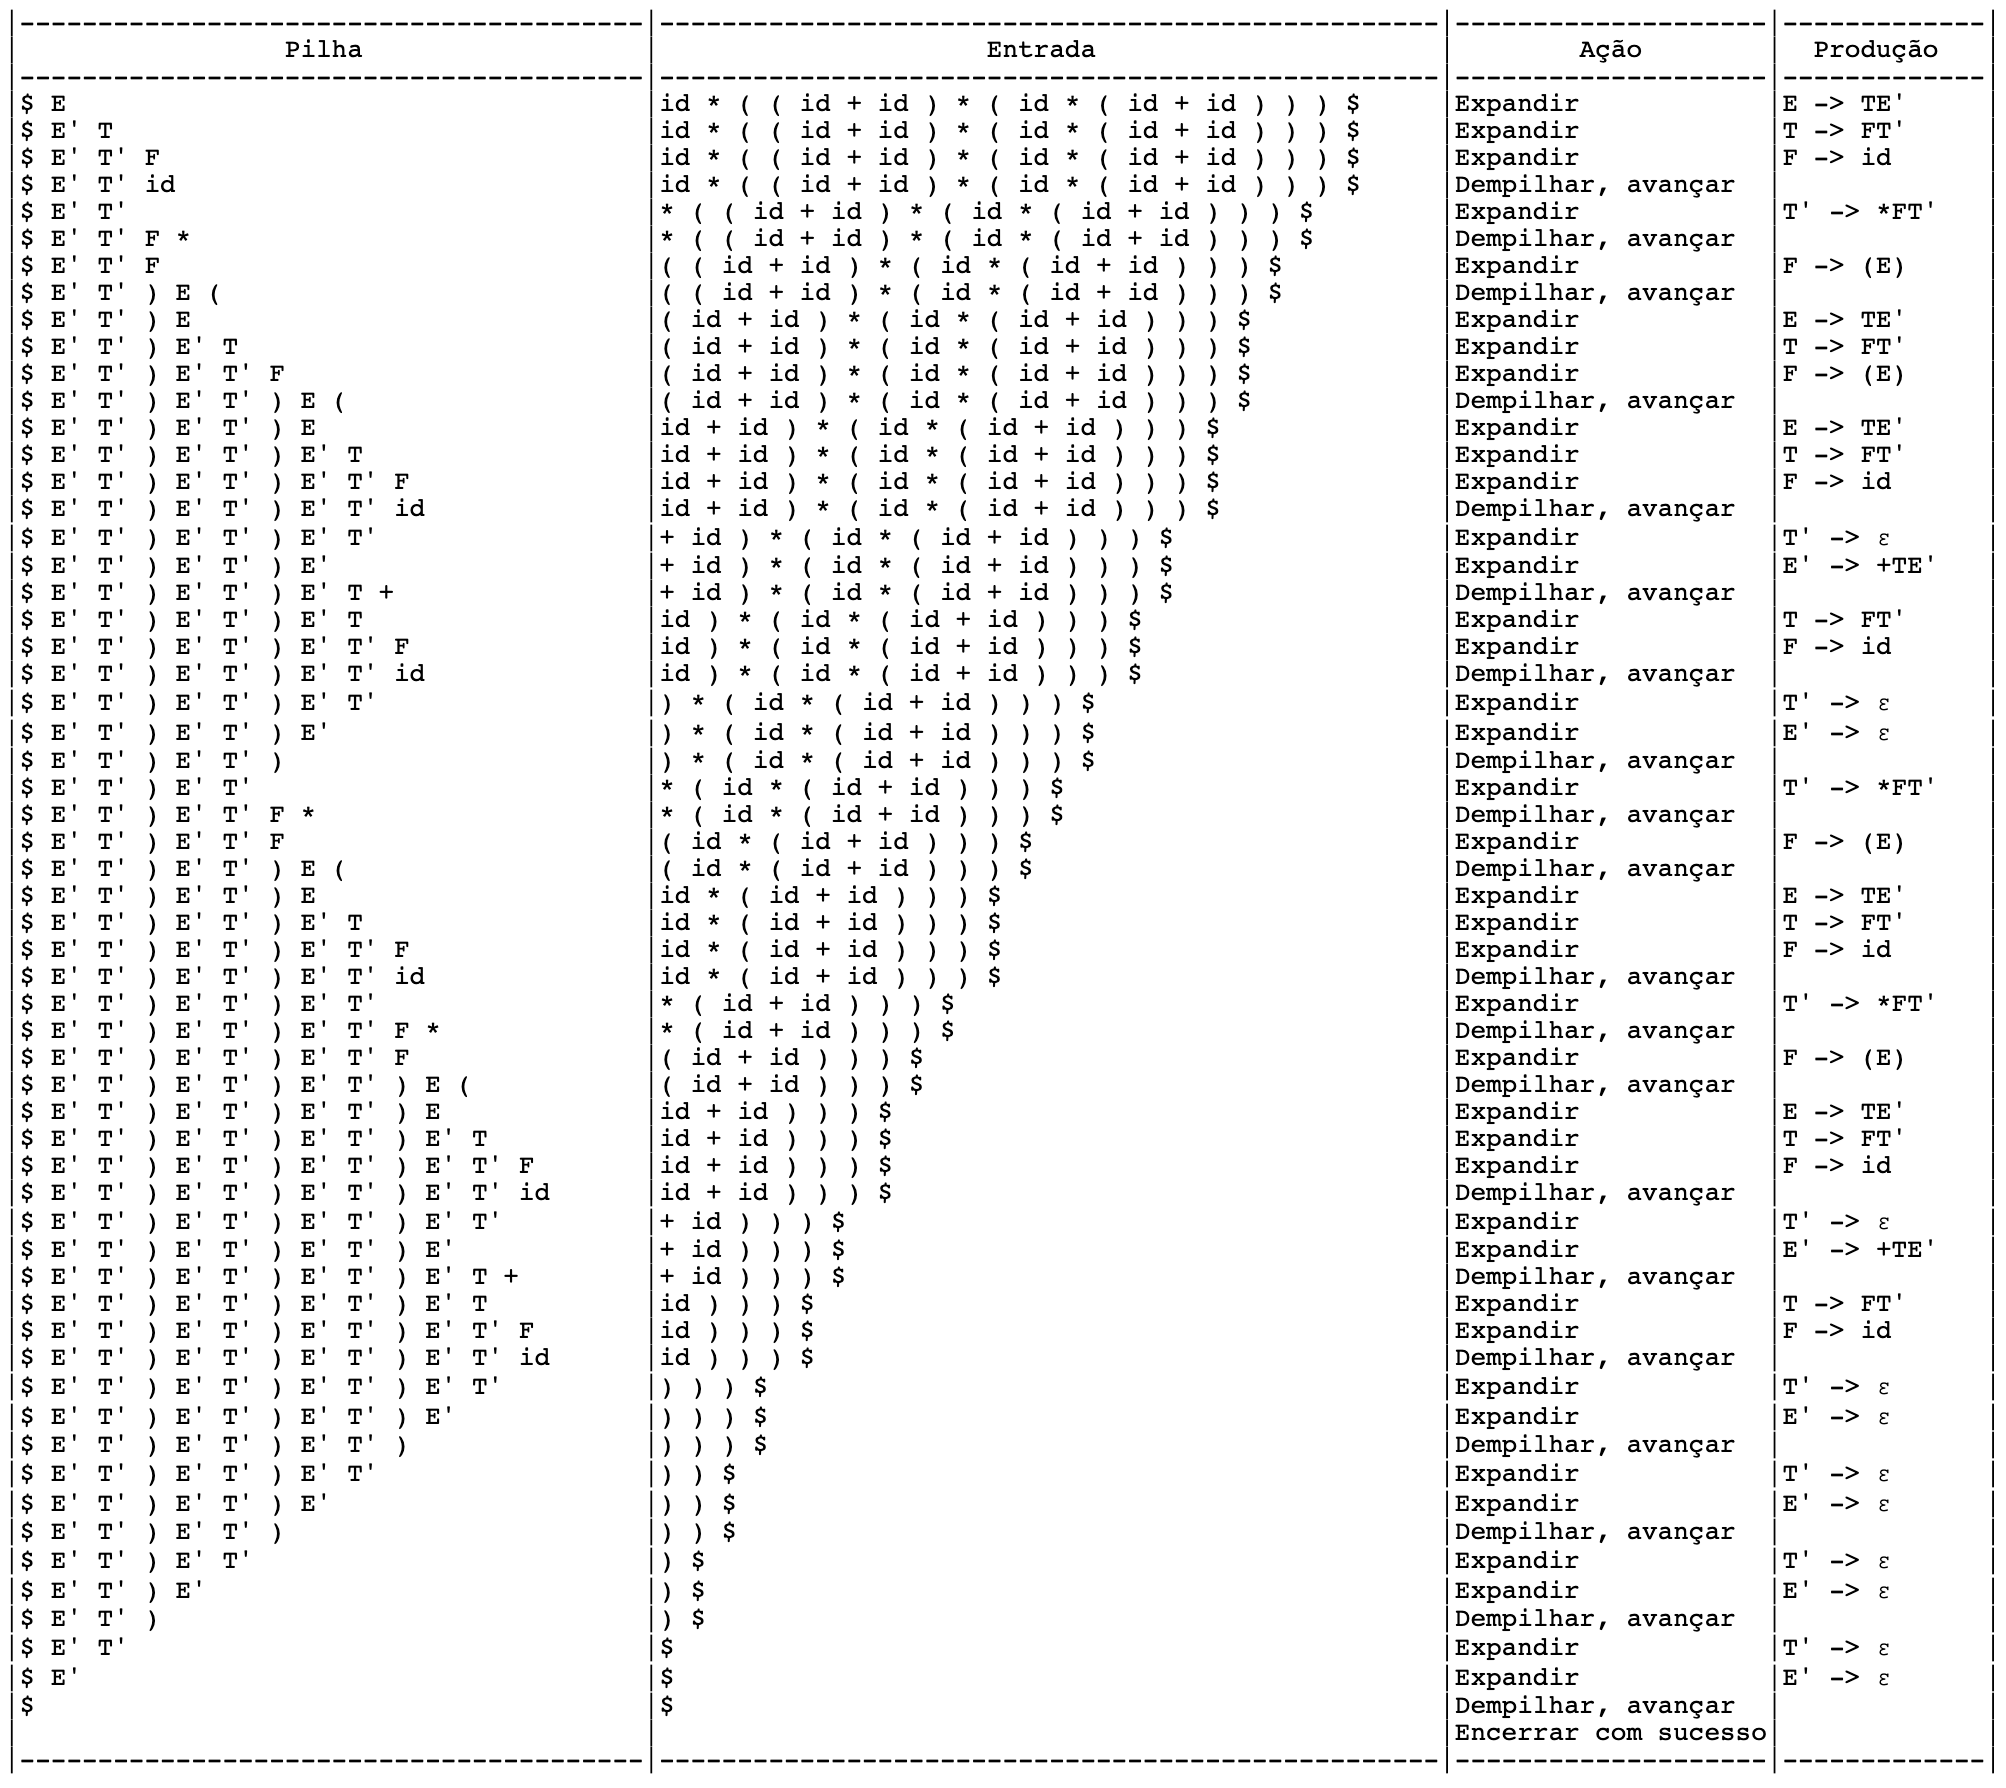
\includegraphics[width=\linewidth]{./../output/output_question2_list_1.png}
  \caption{A tabela de execução para entrada $id * ((id + id) * (id * (id + id))) \$$}
  \label{fig:ouput2}
  \end{center}
\end{figure}

\section*{Exercício 2}

O Exercício foi resolvido com sucesso. Para a gramática do exemplo da Seção 5.4.4 do Capítulo V dos Slides Teóricos de CES-41 e a tabela de produções de um analisador preditor não-recursivo, no mesmo exemplo, foi feita a tabela de execução simulando a análise da sentença $id * ((id + id) * (id * (id + id))) \$$. A tabela de execução pode ser vista na Figura \ref{fig:ouput2}.

\section*{Exercício 3}

O Exercicio foi resolvido com sucesso. A tabela de produções do analisador sintático preditor não-recursivo foi feita com sucesso. O Primeiro de cada símbolo pode ser visto na Figura \ref{fig:quest31}. O Seguinte pode ser visto na Figura \ref{fig:quest32}. A tabela dos Primeiros e Seguinstes pode ser vista na Figura \ref{fig:quest33}. A tabela de produções do analisador sintático preditor não-recursivo pode ser vista na Figura \ref{fig:quest34} inteira. Devido à sua largura, ela foi separada em dividida em seguimentos em apresentada da Figura \ref{fig:quest35} à Figura \ref{fig:quest38} de modo a facilitar a visualização.

% \lstinputlisting[
%     language=c,
%     caption={Código intermediário livre de quádruplas de operadores NOP e de operadores de atribuição desnecessários},
%     label={code:intermediario},
%     style=cppStyle,
%     numbers=none,
% ]{./../list2_question3_answer.txt}

\begin{figure}
  \begin{center}
  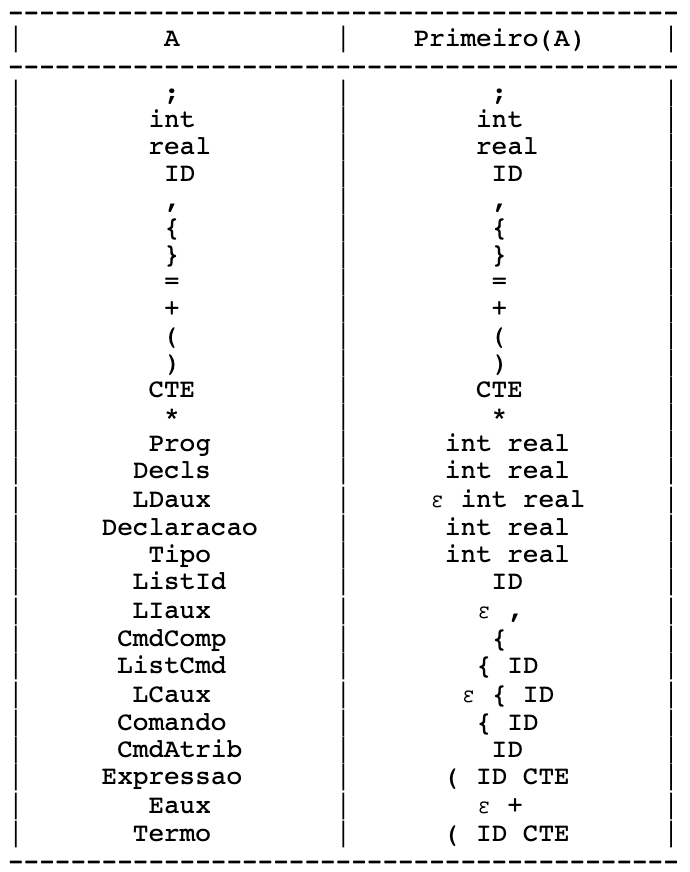
\includegraphics[width=2.8in]{./../output/quest31.png}
  \caption{Tabela dos Primeiros}
  \label{fig:quest31}
  \end{center}
\end{figure}

\begin{figure}
  \begin{center}
  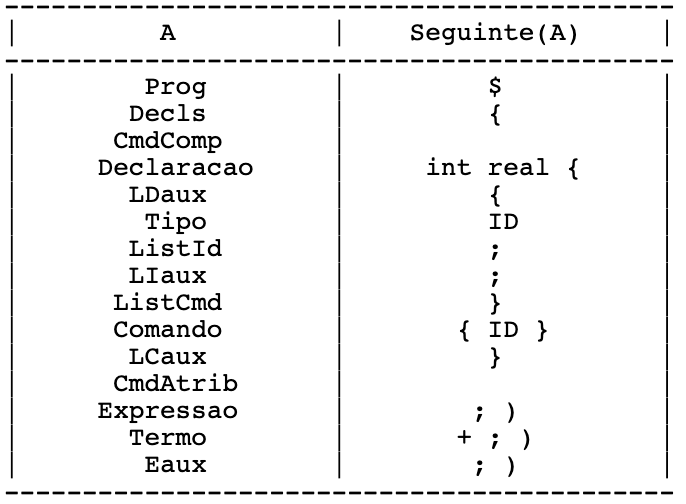
\includegraphics[width=2.8in]{./../output/quest32.png}
  \caption{Tabela dos Seguintes}
  \label{fig:quest32}
  \end{center}
\end{figure}

\begin{figure}
  \begin{center}
  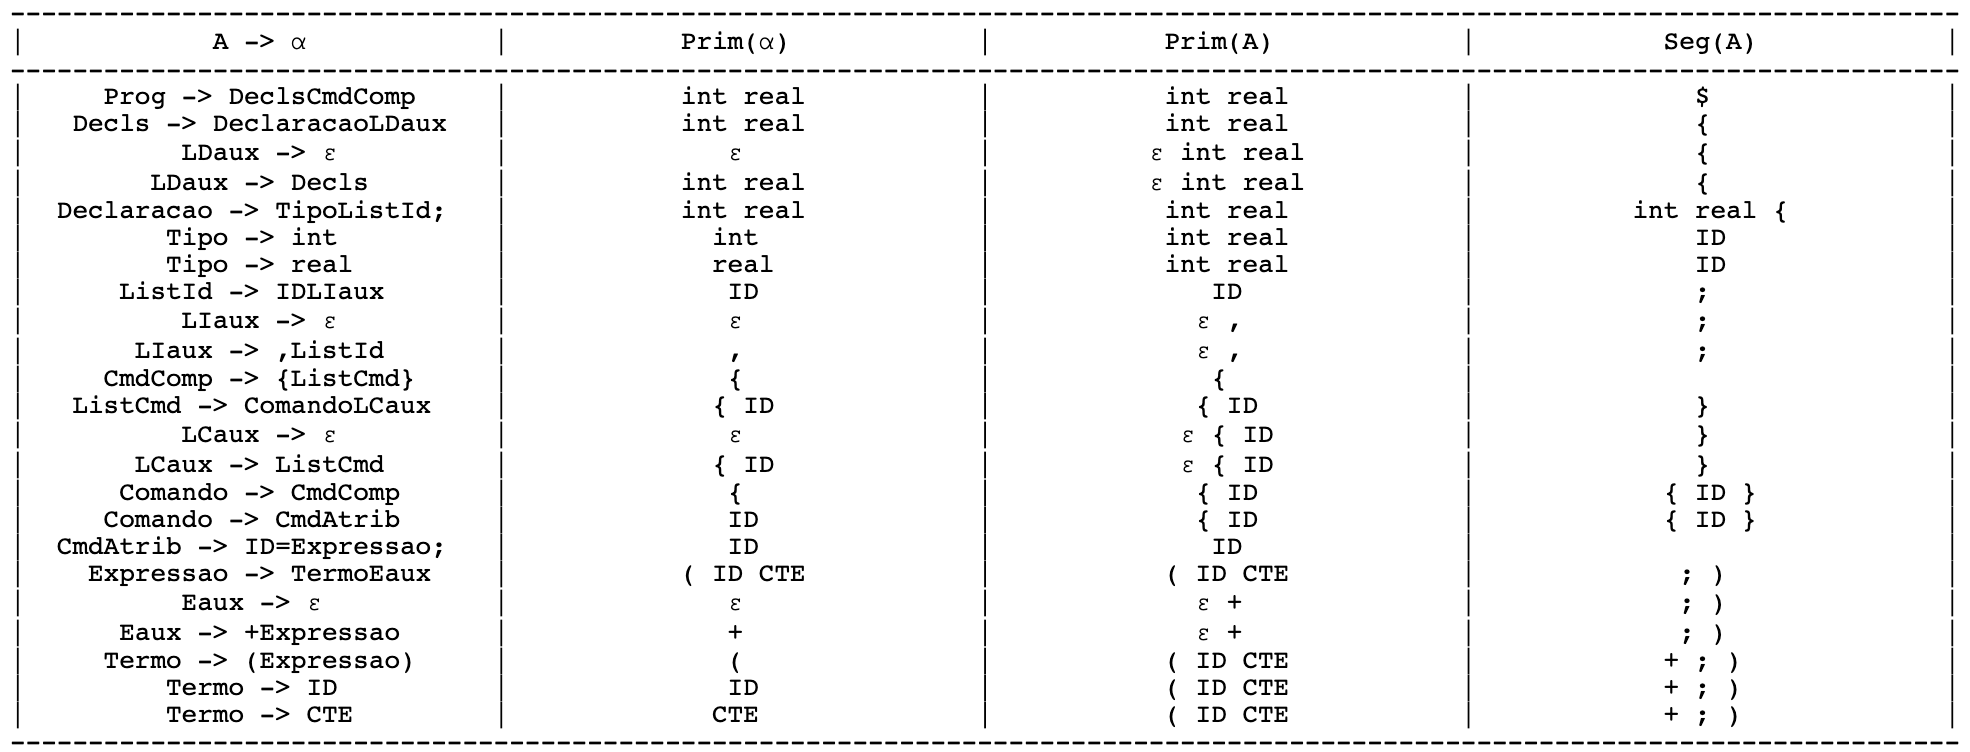
\includegraphics[width=\linewidth]{./../output/quest33.png}
  \caption{Tabela dos Primeiros e Seguintes}
  \label{fig:quest33}
  \end{center}
\end{figure}

\begin{figure}
  \begin{center}
  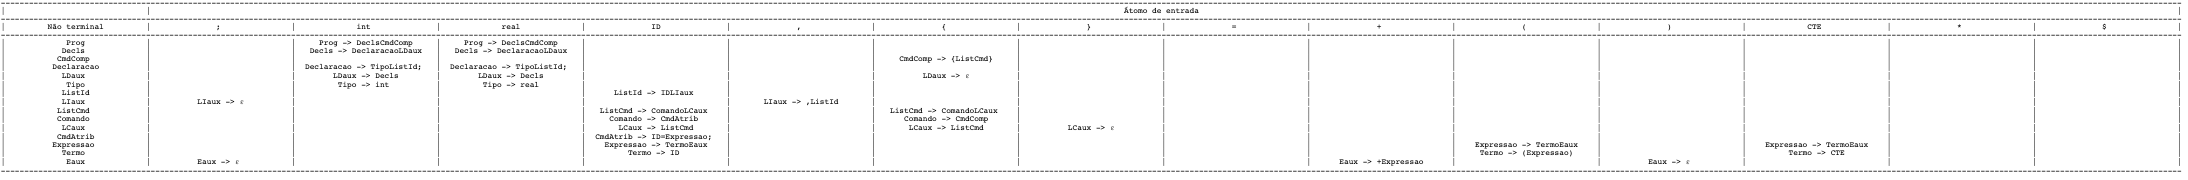
\includegraphics[width=\linewidth]{./../output/quest34.png}
  \caption{Tabela de produções}
  \label{fig:quest34}
  \end{center}
\end{figure}

\begin{figure}
  \begin{center}
  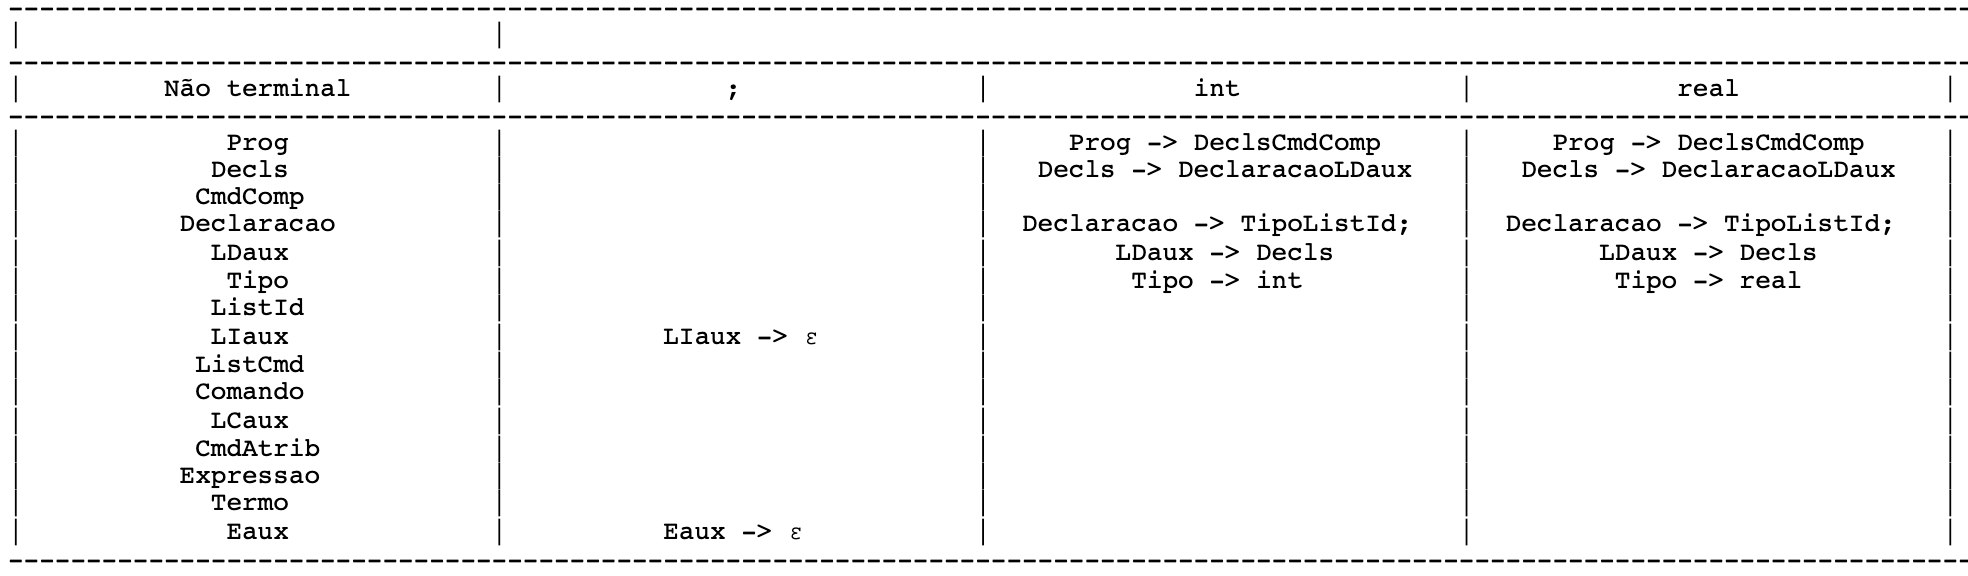
\includegraphics[width=\linewidth]{./../output/quest35.png}
  \caption{Tabela de produções, parte 1}
  \label{fig:quest35}
  \end{center}
\end{figure}

\begin{figure}
  \begin{center}
  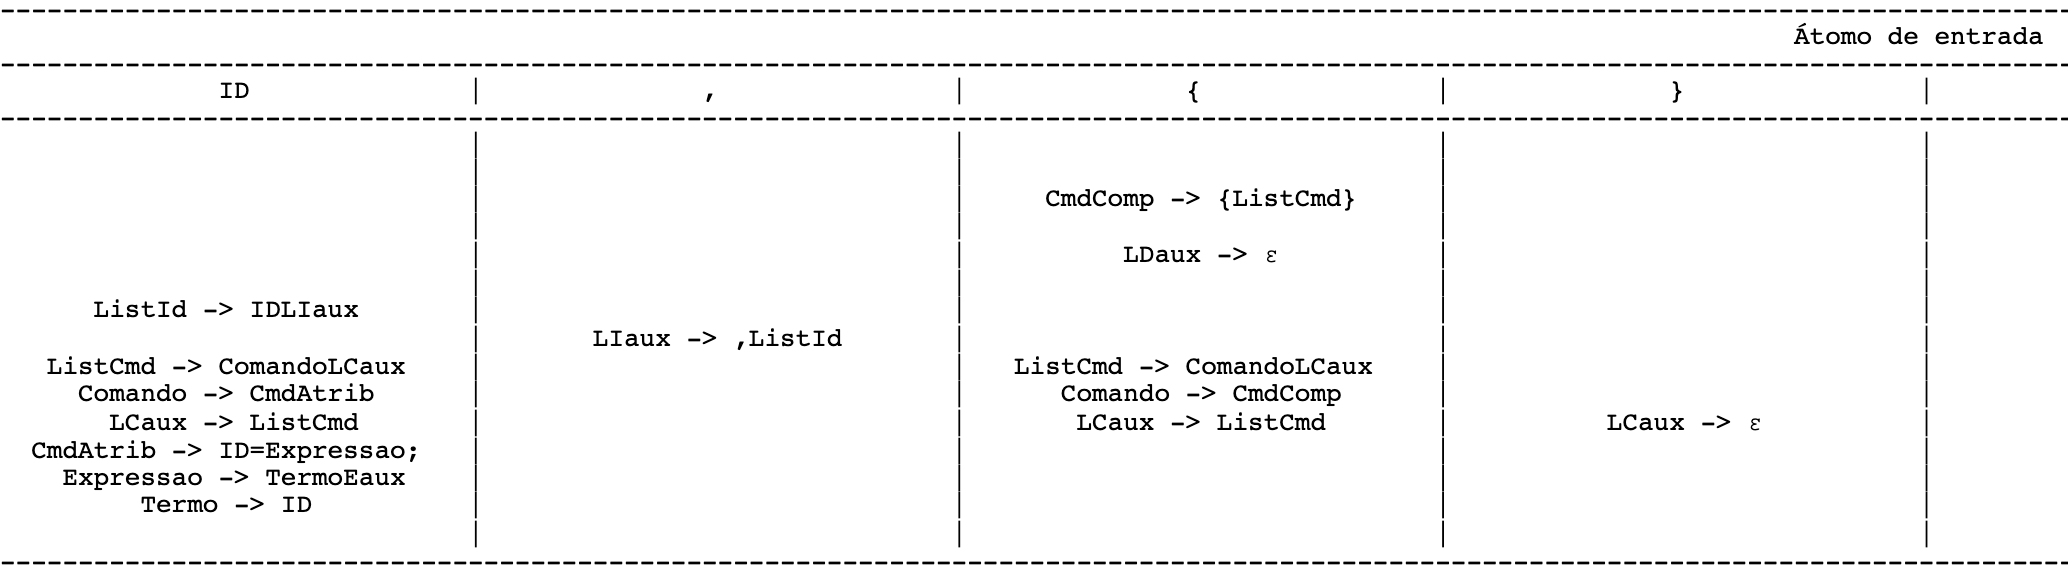
\includegraphics[width=\linewidth]{./../output/quest36.png}
  \caption{Tabela de produções, parte 2}
  \label{fig:quest36}
  \end{center}
\end{figure}

\begin{figure}
  \begin{center}
  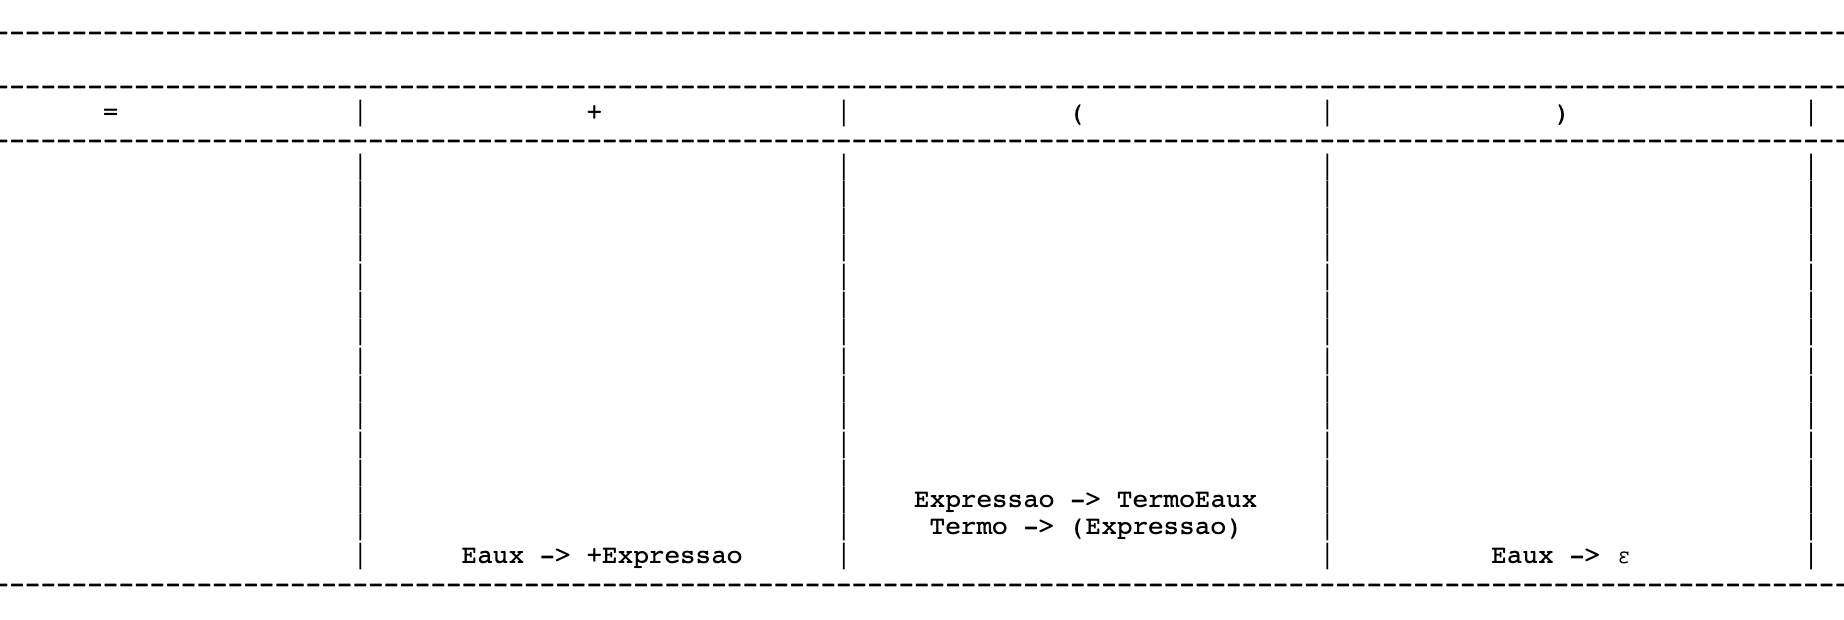
\includegraphics[width=\linewidth]{./../output/quest37.png}
  \caption{Tabela de produções, parte 3}
  \label{fig:quest37}
  \end{center}
\end{figure}

\begin{figure}
  \begin{center}
  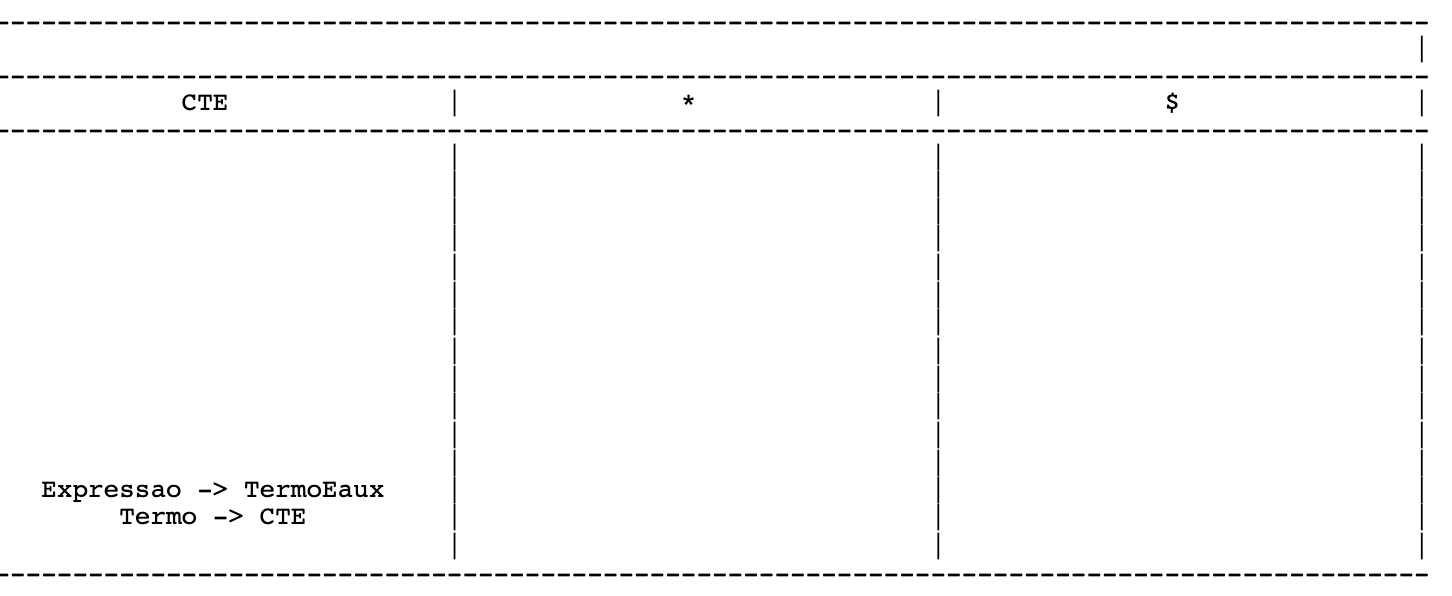
\includegraphics[width=\linewidth]{./../output/quest38.png}
  \caption{Tabela de produções, parte 4}
  \label{fig:quest38}
  \end{center}
\end{figure}

%------------------------------------------------------------------------------

\lstinputlisting[
    language=c,
    caption={Código de entrada para o analisador},
    label={code:entrada},
    style=cppStyle,
    numbers=none,
]{./../input/input}

\lstinputlisting[
    language=c,
    caption={Código de saída do analisador},
    label={code:saida},
    style=cppStyle,
    numbers=none,
]{./../output/output}

\end{document}
